%%%%%%%%%%%%%%%%%%%%%%%%%%%%%%%%%%%%%%%%%
% Journal Article
% LaTeX Template
% Version 1.4 (15/5/16)
%
% This template has been downloaded from:
% http://www.LaTeXTemplates.com
%
% Original author:
% Frits Wenneker (http://www.howtotex.com) with extensive modifications by
% Vel (vel@LaTeXTemplates.com)
%
% License:
% CC BY-NC-SA 3.0 (http://creativecommons.org/licenses/by-nc-sa/3.0/)
%
%%%%%%%%%%%%%%%%%%%%%%%%%%%%%%%%%%%%%%%%%

%----------------------------------------------------------------------------------------
%	PACKAGES AND OTHER DOCUMENT CONFIGURATIONS
%----------------------------------------------------------------------------------------

\documentclass[twocolumn]{article}

\usepackage{blindtext} % Package to generate dummy text throughout this template 

\usepackage[sc]{mathpazo} % Use the Palatino font
\usepackage[T1]{fontenc} % Use 8-bit encoding that has 256 glyphs
\linespread{1.0} % Line spacing - Palatino needs more space between lines
\usepackage{microtype} % Slightly tweak font spacing for aesthetics


\usepackage[english]{babel} % Language hyphenation and typographical rules

\usepackage[hmarginratio=1:1,top=32mm,columnsep=20pt]{geometry} % Document margins
\usepackage[hang, small,labelfont=bf,up,textfont=it,up]{caption} % Custom captions under/above floats in tables or figures
\usepackage{booktabs} % Horizontal rules in tables

\usepackage{lettrine} % The lettrine is the first enlarged letter at the beginning of the text
\usepackage[titletoc,toc,title]{appendix}

\usepackage{enumitem} % Customized lists
\setlist[itemize]{noitemsep} % Make itemize lists more compact

\usepackage{abstract} % Allows abstract customization
\renewcommand{\abstractnamefont}{\normalfont\bfseries} % Set the "Abstract" text to bold
\renewcommand{\abstracttextfont}{\normalfont\small\itshape} % Set the abstract itself to small italic text

\usepackage{titlesec} % Allows customization of titles
\renewcommand\thesection{\Roman{section}} % Roman numerals for the sections
\renewcommand\thesubsection{\roman{subsection}} % roman numerals for subsections
\titleformat{\section}[block]{\large\scshape\centering}{\thesection.}{1em}{} % Change the look of the section titles
\titleformat{\subsection}[block]{\large}{\thesubsection.}{1em}{} % Change the look of the section titles

\usepackage{fancyhdr} % Headers and footers
\pagestyle{fancy} % All pages have headers and footers
\fancyhead{} % Blank out the default header
\fancyfoot{} % Blank out the default footer
\fancyhead[C]{Practical MA-ABE for Secure Cloud Storage Systems $\bullet$ August 2018 $\bullet$ Vol. I, No. 2} % Custom header text
\fancyfoot[EL]{\thepage} % Custom footer text

\usepackage{titling} % Customizing the title section

\usepackage{hyperref} % For hyperlinks in the PDF
\usepackage{multicol}
\usepackage{graphicx}
\usepackage{caption}
\usepackage{amsmath}
\usepackage[textsize=footnotesize]{todonotes} % for todo notes

% define new command for \req (bold and italic)
\newcommand{\req}[1]{\textbf{\textit{#1}}}

% use \todo[inline] per default
\let\originaltodo\todo
\renewcommand{\todo}{\originaltodo[inline]}

\newcommand{\question}[1]{\originaltodo[color=green, inline]{#1}}

%----------------------------------------------------------------------------------------
%	TITLE SECTION
%----------------------------------------------------------------------------------------

\setlength{\droptitle}{-5\baselineskip} % Move the title up

\pretitle{\begin{center}\Huge\bfseries} % Article title formatting
\posttitle{\end{center}} % Article title closing formatting
\title{Practical Multi-Authority Attribute-Based Encryption Scheme for Secure Cloud Storage Systems } % Article title
\author{%
\textsc{Marvin Petzolt}\\[1ex] % Your name
\normalsize TU Berlin \\ % Your institution
\normalsize \href{mailto:marvin.petzolt@protonmail.com}{marvin.petzolt@protonmail.com} % Your email address
%\and % Uncomment if 2 authors are required, duplicate these 4 lines if more
%\textsc{Jane Smith}\thanks{Corresponding author} \\[1ex] % Second author's name
%\normalsize University of Utah \\ % Second author's institution
%\normalsize \href{mailto:jane@smith.com}{jane@smith.com} % Second author's email address
}
\date{\today} % Leave empty to omit a date
\renewcommand{\maketitlehookd}{%
\begin{abstract}
If a group of users want to share a ciphertext, they need to agree on a shared key. In order to ensure forward and backward secrecy, this shared key needs to be updated and distributed to every member everytime a user leaves or joins the group. Classical encryption methods encounter their limits, in which this approach is no longer feasible for a large number of users. In this work the field of attribute based encryption (ABE) will be analyzed to solve this issue for a secure cloud storage environment (Bdrive). Different ABE schemes will be compared for their applicability in Bdrive. Finally, the implementation of the resulting scheme will be evaluated for performance, scalability and security.
\end{abstract}
}

%----------------------------------------------------------------------------------------

\begin{document}

% Print the title
\twocolumn[
    \maketitle
]


%----------------------------------------------------------------------------------------
%	ARTICLE CONTENTS
%----------------------------------------------------------------------------------------

\section{Introduction}
\label{sec:introduction}
\todo{
	* **Introduction**\\
	* Ruff problem describtion\\
	* How ABE can solve this\\
	* How ABE works\\
	* Short history summary of ABE\\
	* What is expected of this work\\
	* What are the targets
}
\lettrine[nindent=0em,lines=3]{I}n public-key cryptography each user is identified by his unique public and private key pair. Peer-to-peer communication works well with this scheme, but as soon as an encrypted content needs to be accessed by multiple participants, the data owner has to encrypt the content for each user explicitly. This results in many encrypted versions of the same  file, each secured by a different public key. Such scheme does not scale in the secure cloud storage domain. Here often data holders want to share the same content with many other users at the same time.

We reach the point where the classical public-key end-to-end encryption scheme does not scale anymore. We would like to employ an encryption scheme which has a constant number of access keys regardless of the number of participants.

\section{Related Work}
\todo{
	* **Related work**\\
	* Of paper did something similar to this\\
	* Comparison paper\\
	* Not ABE paper
}

\todo{
	Cite \cite{lee2013survey} and similar overview paper
}

\subsection{Attribute-Based Encryption}
Attribute Based Encryption (ABE), first introduced by Sahai and Waters \cite{sahai2005fuzzy}, is a cryptographic encryption scheme which uses attributes of a user as keys for encryption. This enables the data owner to craft a ciphertext over chosen attributes that can only be decrypted by any entity that holds a super set of matching attributes. Further, it is possible to embed a complex access structure (e.g. access trees) inside the cipher text, where each node contains \textit{AND} or \textit{OR} threshold gates. This approach is known as Ciphertext-Policy Attribute-Based Encryption (CP-ABE) \cite{bethencourt2007ciphertext}. 
It is also possible to do it the other way around: Associate the user's key with an access policy, formally known as Key-Policy Attribute Based Encryption (KP-ABE).\cite{goyal2006attribute}. 
%Now the encryptor needs only to encrypt a given plain text with the public key of specific attributes so that only users who hold the right keys are able to decrypt the cipher text.

Both approaches are limited to one attribute authority (AA). So only one trusted entity is in charge of issuing attributes and their matching key pairs. However, in the real world we would like to distribute the issuing of attributes over different authorities. A new scheme is needed where different attribute authorities cooperate and communicate across different domains.  

% The basic idea is, as proposed in \cite{chase2007multi}, to construct for each users a polynomial of degree $d-1$, where $d$ donates the number of attributes in our system. 

Multi-Authority Attribute Based Encryption (MA-ABE), first proposed by Chase 2007 \cite{chase2007multi}, allows multiple attribute authorities to maintain different attribute domains. To ensure collusion resistance between users, a trusted  Central Authority (CA) was introduced to assign each user an unique identifier (UID) and making the decryption process depending on this UID. Its disadvantage is the CA's global decryption power and therefore the necessity to remain trusted. 
%To prevent collusion between user in a multi authority setting, the challenge for each user needs to be individual. But it still needs to be ensured that the encryption of a message is independent of any user specific identifier, since the encryption progress should sourly depend on the attribute set known to the system.
%To mitigate this problem a global identifier (GID or UID) per users was introduced that is shown to each attribute authority (AA) to receive the corresponding private key for the users attributes. 
%The central authority (CA) now has to make sure that the user dependent challenge results in a global decryption key to decrypt the message.
%In fact the CA has to be trusted since it computes the users private keys in such a way that on decryption it reveals the global decryption key. 
Chase \textit{et al.} addressed this issue in \cite{chase2009improving} by distributing the global secret  master key generation over the AAs. However, since the global master secret is computed on system initialization, no further AAs can be added afterwards without rebooting the system. Also the scheme did not support attribute revocation which rendered it practical not applicable.
% Each authority uses this seed in combination with a pseudo random function to deterministically create the users private key. Since the CA possesses the same seed, same pseudo random function and issues the users GID, it can also compute the same private key as issued by the corresponding AA. So it can ensure that on decryption the keys add up to reveal the global decryption key. This scheme has a major issue: The CA has global decryption power. 

% Chase notices this problem as well and tried to mitigate it by decentrializing the seed generation \cite{chase2009improving}.  First user attributes could not easly be revoked\footnote{Chase proposed to assign each user a range of GIDs, so that a user can migrate to the next GID on revocation. Since the GID range is finite, this solution does not scale.}. Second AA's cant be added on runtime without reissuing each user his keys. And last, the attribute universe is finite (no large-universe). Further we noticed that if a failure of one AA renders the system unresponsible, since a cyphertext includes attributes from each authority. 

Data Access Control for Multi-Authority Cloud Storage Systems (DAC-MACS) \cite{yang2013dac} is a scheme that tackles both of this issues. Each authority receives its own ciphertext that depends solely on the attributes issued in this domain. While Chase managed to maintain the "one-plaintext-one-ciphertext" ratio, DAC-MACS needs to create $k$ ciphertexts: One per AA.\footnote{If the ciphertext does not require any attributes of an specific authority it does not have to create a ciphertext for this domain.} It does not require any coordination between authorities which enables to add new AAs at runtime without recreating the user keys. This scheme also includes features for efficient revocation while it claims to maintain forward and backward secrecy. 

DAC-MACS is not collusion resistance on attribute revocation under the active attack model. The scheme NEDAC-MACS (New Extended DAC-MACS) shows and solves this vulnerability \cite{wu2017security}. Recent studies introduce a more efficient, scalable and secure approaches such as MAACS \cite{li2016secure} and TFDAC-MACS (Two-Factor DAC-MACS)\cite{li2017two}. The DAC-MACS family is further known for the proxy decryption technique, first introduced by \cite{li2013matrix}, where a honest-but-curious server helps the user on decryption.

Priscilla and Nagarajan 2018 \cite{nagarajan2018overview} conducted an analysis of the DAC-MACS family. In addition to that work, this thesis will focus on alternative approaches to improve scalability of secure cloud storage systems and analyze the field of ABE and MA-ABE more deeply.

%------------------------------------------------

\section{Contribution}
\todo{
	* What are the targets\\
	* What makes this work stand out\\
	* What we can gain from this work
}
The target of this work is to find a more scalable solution to the currently enrolled re-keying scheme in Bdrive. The new scheme needs to satisfy the requirements of section \ref{sec:requirements} with respect to multi-company management (each company administrates only its own domain) and inter-company file sharing (it is possible to share files across companies), as well as it should be practically applicable in the real world.

%------------------------------------------------

% Background  / Problem description
\section{A secure cloud storage system: Bdrive}
\todo[inline]{	
	* How does rekeying in bdrive work currently?\\
	* What security targets are covered\\
	* What is adventagous \\
	* Waht is disadventagous
	}
In the following we will describe the encryption scheme currently enrolled in Bdrive and give a rough overview of the existing solutions in the attribute-based encryption domain.

\subsection{Background}
\begin{figure*}[!ht]
\centering
    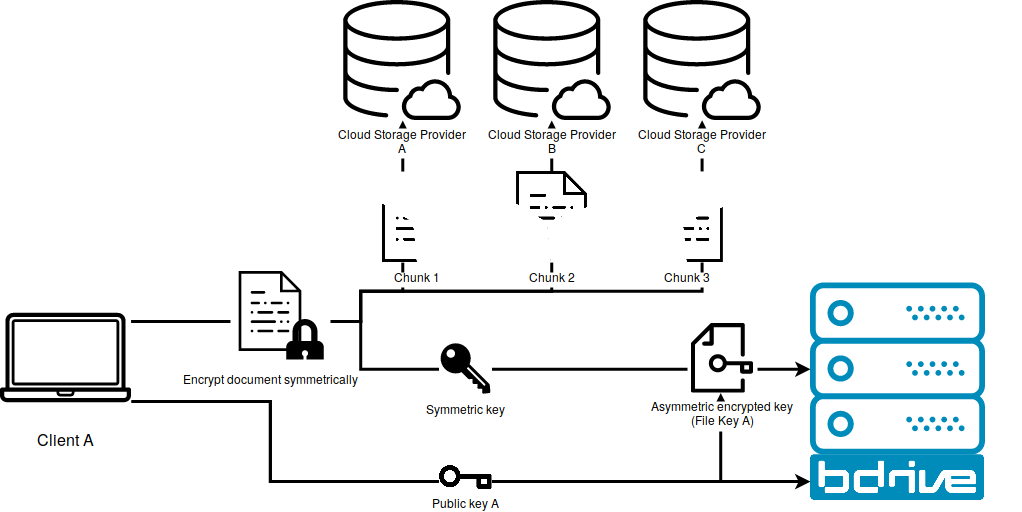
\includegraphics[width=0.8\linewidth]{img/bdrive1.png}\par 
    \caption{Client uploads an encrypted file to the CSPs and the file key and public key to Bdrive.}
    \label{fig:filekey}
\end{figure*}
\begin{figure*}[!ht]
\centering
    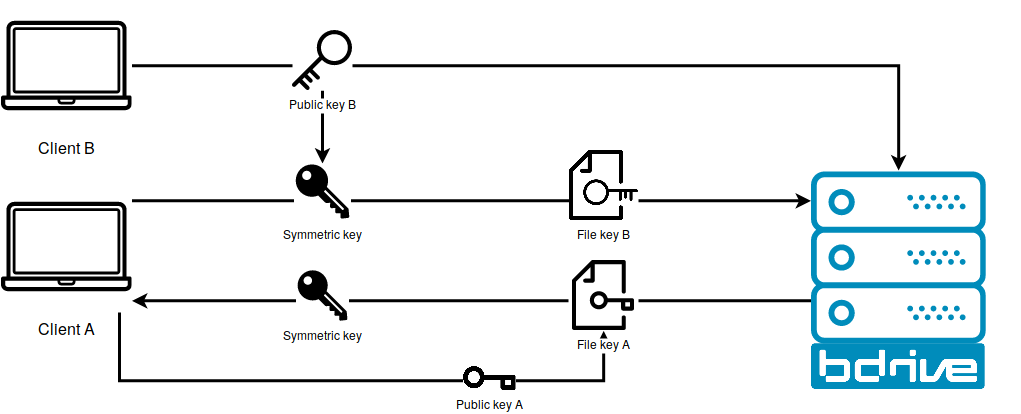
\includegraphics[width=0.8\linewidth]{img/bdrive2.png}\par
    \caption{Client A grants Client B access to the uploaded file by re-keying the file key}
    \label{fig:rekey}
\end{figure*}

Bdrive is a secure cloud storage which splits up files in smaller chunks that are saved separately on different cloud storage provider (CSP). To ensure end-to-end encryption a Bdrive client encrypts locally each of its chunks with a one-time symmetric key that is then encrypted under its own public key. This encrypted key is called a file key and it is uploaded to the Bdrive server where it is stored securely (see figure \ref{fig:filekey}).

Since each device of the same user has a different private-public key pair, the device is in charge of making the file keys accessible for a new device. This will be done by downloading each file key for the respective file, receiving the public key of the new device, decrypting the file key with its own private key, encrypting it again with the public key of the new device and finally, uploading the new file key to the Bdrive server. This process will be called re-keying (see figure \ref{fig:rekey}).

The number of file keys, that need to be maintained in Bdrive, grows linearly with the number of devices. In addition Bdrive allows to share files between different users. For each device of each user involved in a share a new file key has to be created and maintained. 

%The formula \ref{eq:rekey} describes the number of file keys Bdrive that need to be stored for each shared files between $U$ users, where each user $u_{i \in U}$ has $u_d$ devices.

%\begin{equation}
%n = \sum_{i}{d_i}
%\label{eq:rekey} 
%\end{equation}

%Lets construct an example where the manager of a company wants to create a shared folder with all company employees. It is a medium sized company with $50$ employees. Lets assume that at least haft of them have two Bdrive clients running. The manager wants to upload the $250$ photos of the last company trip.
%We end up by computing $3/2 * 50 * 250 = 18750$ file keys and for every new file uploaded $75$ new file keys need to be uploaded. 

\section{Bdrive Rekeying scheme}
\todo[inline]{find better title}

In Bdrive each device of a user generates a new RSA key pair on registaion. The fingerprint (hash) of the public key identifies the device uniquly. To save a file in the cloud the device fist encrypes the file symmetrically with the so called "filekey". The filekey equals the hash of the plain file content and so ensures tamperproofness and integirty on decryption. Since Bdrives supports end-to-end encryption the server should never be able to decrypt the file by itself. So the device encrypts the filekey asymmetrically with its own public key and uploads the filekey to the Bdrive server were it is stored securly. The encrypted file is uploaded to the different cloud storage provider. 

If the user wants to access a file locally, the devices requests the encrypted filekey from the server, downloads the file chunks from the cloud storage providers, decrypts the file key with his privat key and finally decrypts the file with the filekey. 

So far we saw how the encryption process is handled for a single device. However, this process turns out to be much more complex in computation in a multible devices setting.  If a user registers more then one device the exisiting data needs to be syncronized to the new device. The server nodifies the existing device for the new registered device and the public key of the new device is downloaded. Now, each filekey for each file of the user needs to be downloaded from the server and decrypted. To make them accessable for the new devices, they are encrypted with the new devices public key and uploaded again to the server. The new device can now start to download and decrypt the filekeys as decibed previously. 

Some may notice, that this approach is not scalable for a large number of devices. Others may argue that a user never has so many devices that this process is no longer maintanable. But a cloud storage system provides the possibility to share the files with other users. Which means that each device of the user that accepts the invitation to the share needs to have an own encrypted file key. This process scales with $O(n * f)$ keys. Were $n$ donates the number of devices onvolved in the sharing and $f$ the number of file versions in the share.\footnote{Each file consit of many file versions. Each file version needs an own file key since the content changes each time the file is updated.} Futher, we need to send $O(n * f)$ messages to send each device its personal filekey and we need to encrypt each filekey $n$ times which also results in $O(n * f)$ encryptions in total. 

If a new devices joins the share we need to make the existing file keys avaiable to the new devices which results in $O(f)$ additional encryptions, messages and keys. However, a big adventage of this scheme is that we don't have to anything if a member leaves the group. We simply remove all the filekeys belonging to the left device and do not further encrypt new uploaded files for this device. Forward secrey\footnote{Forward Secrecy: The left member do not have any knowledge about future shared content.} is ensured. Backwards secrecy is also provided since a device needs to rekey for the newly joined member to make the files accessable for him. 

How can we do better then this while still maintaining the same level of security? 

\section{Requirements}
\label{sec:requirements}
The general (\textbf{\textit{B*}}) requirements of this thesis will be summarized by two major points: 

\begin{itemize}
	\item[\textit{\textbf{B1}}] \textbf{Performance:} Participating in the system should be possible with low-performance devices (such as smartphones). The overhead for the server on proxy decryption, attribute issuing and revocation should be reasonably low.  
	\item[\textit{\textbf{B2}}] \textbf{Scalability:} The system should scale better than the current encryption scheme with respect to the number of file keys. 
\end{itemize}

In addition, the core (\textbf{\textit{C*}}) security requirements in the context of an MA-ABE scheme are the following:
\begin{itemize}
\item[\textit{\textbf{C1}}] \textbf{Collusion resistance:} For two users it should not be possible to combine their attributes to archieve a higher level of decryption power.
\item[\textit{\textbf{C2}}] \textbf{Inter-Company Sharing:} Each company is only responsible for its own domain. This includes attribute and user administration, which translates to secret key generation and revocation. %Since Bdrive would need to consider a multi-authority ABE scheme, it should not be possible for a company to decrypt or issue files of other companies if no explicit exception is given for certain files by a trusted company relationship. A companies attribute authority (AA) should be responsible for its domain. In the case of an inter company relationship, attributes needs to be issued across different companies. 
\item[\textit{\textbf{C3}}] \textbf{Central Authority:} The CA shall not have global decryption power. At most an AA can decrypt user files of its own domain.  
\item[\textit{\textbf{C4}}] \textbf{Secret Master key (if any):} Key recovery requires a secret and securely stored master key. It should solely function in the company domain and not globally. 
\item[\textit{\textbf{C5}}] \textbf{Large Attribute and Key Universe:} The number of attributes and users shall not be restricted.
\item[\textit{\textbf{C6}}] \textbf{Adding new Attribute Authorities:} It should be possible to add new attribute authorities at runtime. Without either shutting down the system or recreating each key.
\item[\textit{\textbf{C7}}] \textbf{Untrusted Attribute Authority:} A corrupt Attribute Authority can only harm its own domain, but can not harm the outside system in any way. It cannot gain any additional information.
\item[\textit{\textbf{C8}}] \textbf{Key and Attribute revocation:} Revocation is needed to handle user management in terms of attribute promotion, attribute demotion and key revocation. Forward secrecy should be provided. 
\end{itemize}

\noindent Other (optional \textbf{\textit{O*}}) requirements are: 
\begin{itemize}
	\item[\textit{\textbf{O1}}] \textbf{Traitor tracing:} A user in ABE is described by his attribute set and is anonymous in this set. Misbehaving users, who sell their attribute keys to create a decryption black box, should be identifyable. \cite{liu2016practical}
	\item[\textit{\textbf{O2}}] \textbf{Fine-grained access control:} The user shall not be bounded on defining fine-grained access policies which requires either an access tree \cite{bethencourt2007ciphertext} or an linear secret sharing scheme (LSSS) \cite{yang2013dac} \cite{li2016secure} \cite{wu2017security} \cite{li2013matrix} \cite{liu2016practical}.
	%Some schemes restrict the user to threshhold access policies, where an user needs at least $n$ of $m$ attributes to encrypt the cipher text. \cite{chase2007multi} \cite{chase2009improving} Other approaches are restriced to $AND$ gates which would translate to $m$ of $m$ threshhold gates. \cite{li2017two}
\end{itemize}

% Secure group communication
\section{Secure Group Communication}
The most simple approach to this challange is to create a secret \textit{group key} (GK) each time multible devices need to access the same file. This schemes are called "Secure Group Communication" (SGC). The main idea is to reduce the number of filekeys by encrypting all the files with a unique GK that is only known to the members in the share. Very simple approaches use a so called \textit{Key Distribution Center} (KDC) to distribute the group keys to each member. However, while Bdrive could manage forward secrecy quite easily, this schemes suffer from additional rekeying overhead if a member leaves the group. 

% Mutlicast in group communications
Often Secure Group Communications are mentioned together with \textit{multicat messages}. The idea is that on \textit{unicast} a central authority is required that manages authentication and authorization to decide which entity should access which content. With multicast messsages content is distributed to each entity regardless if this entity is authorized to view the content. Authorization is handled via encryption of the content. If an entity owns the key to decrypt the data it is implizity authorized to view the content. Multicast messages are expecially handy in group communciations since we only need to send one message to distribute the information to all members.\todo{sources??, verify if this is true} 

% The role of PKI in group communications
While there are many approaches researching secure group communication and making the process more efficient of rekeying more efficient, we can reduce the number of schemes to thouse applicable to secure could storage. Here some prerequisits are given that are not generally assumed. Secure cloud storage system often deploy a public key infrastrcture (PKI) to bind identities to public keys of clients.

Schemes that extend the 2-parties Diffie-Hellman (DH) key exchange to n-party scheme, such as in \textit{Steiner at. al., 1996}\cite{steiner1996diffie}, are not very adventurous in a PKI environment. The DH key exchange is designed for unsecured environments to create a unique communication key, known to every member in the group, but not known to a passive attacker. However, since we can assume that all communication is already disclosed and secured by the PKI we can elimate thouse schemes. They suffer from additional computation or message exchange overhead compared to schemes that assume an existing PKI.   

In the following it will widly assumed that a client is identified uniquly by its public key, which is also known by the cloud server and can be queried by other clients. 

\subsection{Group Key Management Protocol}
The Group Key Management Protocol (GKMP)\cite{harney1997group} addresses this issue in a simple but more scalable way. If a device want to share files with a group it creates the group key and encrypts all filekeys with this group key. This GK needs to be securly distributed to all members which means that the data owner needs to download and store every public key of the group members and encrypt the GK for each of them. Further, the data owner needs to encrypt all shared filekeys symmetrically with the chosen group key. 

% Disadventage
To ensure forward secrecy, the GK needs to be renewed everytime a member leaves the group. This process is located in the same computational magintude as bootstrapping a new group. 

% Adventage
The big adventage of this scheme, compared to the scheme employed in Bdrive, is that it recudes the overhead of encryptions, messages and keys on new file uploads dramastically. While the data owner had to create a filekey for each member respectivly, GKMP reduces this to one filekey per upload. Additionally, since we don't have to ensure backward secrecy, we only have to distribute the GK to the new joind member.

\subsection{Logical Key Hirachy}
\begin{figure*}[!ht]
\centering
    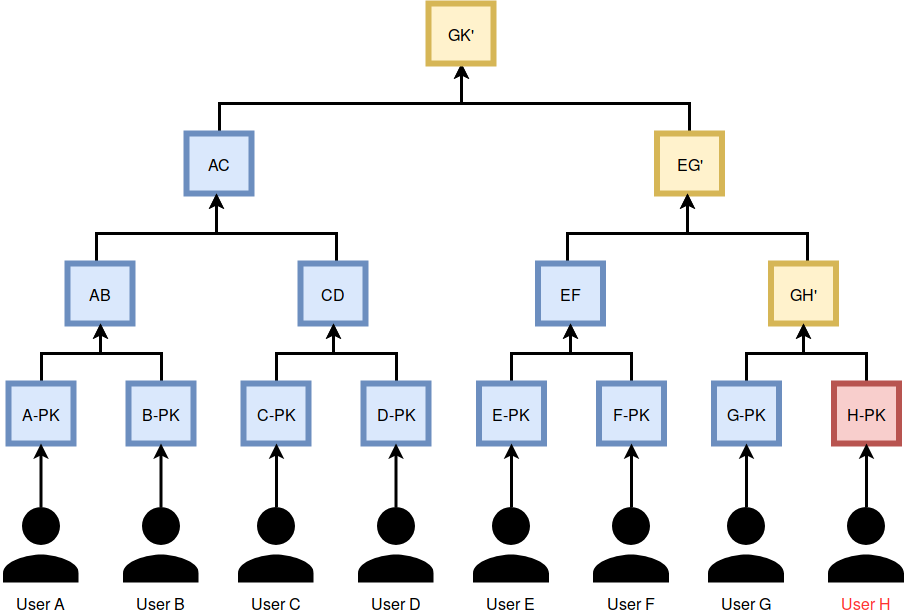
\includegraphics[width=0.8\linewidth]{img/LKH.png}
    \caption{Balanced binary LKH and \textbf{User H} joins or leaves the group. Node marked in yellow is newly added to the group. Node marked in green require an update and need to be stored locally by the user.}
    \label{fig:lkh}
\end{figure*}
\todo{fix image placement}

Logical Key Hirachy (LKH)\cite{wallner1999key} is a GKMP that reduces user side storage and rekey-tranmissions by organizing users keys in a tree hirachy and maximaly exploiting the use of multicast messaging. The whole tree is mainted by a central \textit{Key Distribution Center} (KDC). In the litrature it is explicitly stated that this trees neither habe to be balanced nor binary, but for the sake of simplity excatly this is assumed. Users (and their respecitv public keys) are organized on the lealf if this tree. Each node is composed of a key that is encrypted respectivly with its children keys. This encrypted key is known to all leafts related to this node and can, on change of this node, be transmitted in one multicast transmission to all its leafs. The root node summarizes the GK. The GK is used in the same way as in GKMP to secure the group communication. 

While in GKMP each user needs to store each members public key to eventually rekey the group, in LKH each user only needs to store $log(n) +1$ keys (path from leaf to root node). Beginning from the buttom each leaf node could decrypt the next parent node until it arrive at the root node. The other adventage is that many members share the same keys. So it is more efficient to transmit this keys in a multicast setting. LKH needs to do $2log(n)$ multicast transmissions and analogous $2log(n)$ encryptions on each member leave or join.  Here each updated key in the path from leaf to root node needs to be updated and encrypted two times: One time with the key of right children node and second with the key of the left children node. 

In figure \ref{fig:lkh} user H recently joined the group which means, that to ensure backward secrecy, the keys in node $GH$, $EG$ and $GK$ must be updated. The key server will choose a new $GH'$, $EG'$ and $GK'$ and encrypts and distributes them in a buttom up fashion starting by $GH'$. $GH'$ is encrypted with user Gs and user Hs public key (G-PK, H-PK) and send to them. Next, user E and F receive in a multicast transmission $EG'$, which is encrypted with EF and user G and H receive in a multicast transmission $EG'$ which is now encrypted with the newly established $GH'$ key. Finally, GK needs to be updated. $GK'$ is encrypted with AC to multicast transmit it to the users A, B, C and D. And $GK'$ is encrypted with $EG'$ to transmit it in one message to user E, F, G and H. In the similar fashion a user would be added to the tree. Forward secrecy is implicitly given and not easly to remove from this scheme.

\subsection{One-way function trees}
To reduce the transmission and encryption overhead of $2log(n)$ to even further to $log(n)$ other schemes use pheudorandom functions \cite{canetti1999multicast} or one-way functions \cite{sherman2003key} to compute the required keys in the path. This schemes are strongly related to merkel trees, since each update of the user set, will force an update of the root node, the group key.

Each user stores a blinded key for each siblings node in the path to the root node. Starting from the individual key, a user can compute the blinded version of his key. To compute the next parent key, a user uses his blinded key, together with the siblings blinded key, which is feeded into a one way function to create the key for the parent node. This node needs to be blinded to serve as the input for the next level. In such way the user can compute the needed keys up to the GK. 

Lets assume user H joined the group in figure \ref{fig:lkh} and given a crypographically secure hash function $h$. First, user H needs to receive the blinded keys, $h(AC)$, $h(EF)$ and $h(G-PK)$ which he stores locally in addition to his own public key $H-PK$. One-way function trees has the same storage overhead as LKH with $log(n) + 1$.  As already known from LKH, we need to update $GH$, $EG$ and $GK$. This nodes are computed from their children blinded values using a merging function $m$ which takes two inputs and procues one output. This could for example be the concatination of both inputs and then applying $h$ to receive a fixed length output value. Starting from the button,  $GH'$ is computed as $m(f(G-PK), f(G-PK))$, analogous $EG' = m(f(EF), f(GH'))$ and finally the updated group key $GK' = m(f(AG), f(EG')$. The new blinded keys are distributed to their respective users using multicast transmissiong, reducing the transmission and encryption overhead to $log(n)$. Again backward secrecy is implicitly given by the natural update process of each node.


\subsection{Comparison}
\todo{find better title}  

\begin{table*}[!ht]
\centering
\begin{tabular}{l 		| l 						| l 							| l 						| l 						| l }
 						& \textbf{Bdrive}			& \textbf{GKMP}					& \textbf{LKH}				& \textbf{OWFT} 			& \textbf{GDH.1}\\
\hline
\textbf{inizial share} 																																		\\
keys 					& $nf$	 					& $1$  							& $n-1$  					& $n$	 					& $1$ 			\\
messages (unicast)		& $nf$	  					& $n$ 							& $n(log_2(n) + 1)$ 		& $2n(log_2(n) + 1)$		& $2(n - 1)$	\\
messages (multicast) 	& $nf$	 					& $n$ 							& $log_2(n) + 1$ 			& $n - 2$ 					& $2(n - 1)$ 	\\
encryptions				& $nf$	 					& $f + n$ 						& $f + n -1$				& $f + n -1$				& $f + n$		\\
\hline
\textbf{member join} 																																		\\
keys 					& $f$   					& $1$  							& $3 log_2(n)$				& $log_2(n)$				& $1$			\\
messages (unicast)		& $f$  						& $1$			 				& $2(n - 1)$				& $n$  						& $2(n - 1)$	\\
messages (multicast) 	& $f$ 	 					& $1$ 		 					& $2 log_2(n)$				& $log_2(n)$				& $2(n - 1)$	\\
encryptions				& $f$  						& $f + 1$		 				& $f + 2(log_2(n))$ 		& $f + log_2(n)$			& $f + 2$	 	\\
\hline
\textbf{member leave}																																		\\
keys 					& $0$						& $1$			  				& $3 log_2(n)$				& $log_2(n)$				& $1$			\\
messages (unicast)		& $0$						& $n$			 				& $2(n - 1)$ 				& $0$	  					& $2(n-1)$		\\
messages (multicast)	& $0$						& $n$			 				& $2 log_2(n)$				& $log_2(n)$				& $2(n-1)$		\\ 
encryptions 			& $0$						& $f + n$ 						& $f + 2 (log_2(n))$ 		& $f + log_2(n)$	 		& $f+n$			\\
\hline	
\textbf{addition of filekey}																																\\
keys 					& $n$		 				& $0$							& $0$	 					& $0$		 				& $0$			\\
messages (unicast)		& $n$		 				& $0$	 						& $0$ 						& $0$		 				& $0$			\\
messages (multicast)	& $n$ 						& $0$ 							& $0$ 						& $0$	 					& $0$			\\
encryptions				& $n$ 						& $1$ 							& $1$ 						& $1$		 				& $1$			\\
\hline
\end{tabular}
\caption{Comparison of secure group communication schemes. $n$ donates the number of members, $f$ the number of file keys. Backward secrecy is ensured in each scheme. Assuming a balanced binary tree as in figure \ref{fig:lkh}}
\label{tab:comparisons}
\end{table*}

The following table will compare the discussed schemes against each other regarding number of keys, messages, and ecnryptions on inizialisation of the group, when a member joins or leaves and on addition of a new file. 

It is assumped that clients already downloaded the public keys of their desired group members. Backward secrecy need to be ensured every time a member leaves the group.
Further, messages in table \ref{tab:comparisons} are transmissions that contain a key. There are also meta messages that nodify the members about a new file upload or the removal of a member, etc. They are left out since they add a contant overhead to all schemes.  If a message could be processed by multible communication partners we only need to send the message once, in a multicast transmission.

Some cloud clearly see that Bdrives scheme is not optimal at all compared to the different approaches. In fact Bdrive has the worst perforamnce on inizialisation, addition of a filekey and on average also on member join. In general we can assume that $f > n$ since people tend to have more files then members in a share. However, Bdrive has great performance on member leave since client simply don't encrypt anymore for the left member.

It is hard to extract a clear winner. Each of the schemes have their own strength and weaknesses. GKMP has the best inizialisation overhead and OWFT the best rekeying overhead. We can clearly extract from the table that all secure group schmes perform better on filekey upload. Bdrive needs to distribute the new key encryption filekey to $n$ devices. On the other hand the GK only needs to encrypt the filekey once. Automatically all members have access to the new filekey. 

Under the assumption that do not need backward secrey, we select GKMP the most performant candidate. It has great inizialisation overhead is easily understandable and profits from the fact that we do not need backward secrey on member join. LKH and OWFT both do not get better performance if we remove the backward secrecy constain since this security feature is deeply implemetned in the design of thouse schemes. 

% solution: ABE
\section{An introduction to the field of Attribute-Based Encryption}


\subsection{Identity Based Encryption}
The idea of using universal identifier instead of public keys to identify individuals goes back until 1984. Shamir proposed in \cite{shamir1984identity} to use a central authority to create for each newly registered user a unique universal identifer (e.g. an email address) that can be used for encyrption as we used to do with a public key. However, the difference to RSA is that since the universal identity \textit{is} the public key the use of a PKI becomes insignificant\todo[inline]{find better word to insignificant}. A central authority was introduced since the users private key are dirrived from a random seed only known to this authority. If this seed was publicly known each user could simply compute the private key from any public identifier and so confidentallity would be broken. 

Since this scheme could neither be shown to be practical applicable, nor to proven secure, it was not until 2001 when Boneh and Franklin proposed in \cite{boneh2001identity} a new approach to identity based encryption. The use of the \textit{Weil pairing} revelutionzied the field of identity based encryption.\footnote{Currious reader can readup on the weil pairing here \cite{Miller2004} \cite{galbraith2008pairings} or here \url{https://medium.com/@VitalikButerin/exploring-elliptic-curve-pairings-c73c1864e627}}

\todo[inline]{How does this relate to ABE. Features of ABE}


To go beyond the limitations of secure group communications a different approach to this problem is needed. Lets take a step back and look at groups communications from another perspective then from the cryptographic side. How are groups composed? How are they formed and how is chosen who participates? 

\subsection{Relationship between groups and attributes}
Group in general summarize a specific group of individuals. Specific in that kind, that key share a common feature. In a company, for example, groups are based on shared attributes such as "working in the same team", "working in the same company" or "dinkes coffee". The more common use case, at least in the businesss area, is that users want to distribute content to groups rather then people. This means that if Alice wants to send an encrypted file to the management office she does not care which manager decrypts her file. Everyone in the deparment should be able to do so. 

\subsection{Comparing Secure Group Communication to Attribute-Based encryption}
Comparing SGC to ABE is non tivial. This is due to a different encryption technique used by ABE: paring. Pairing scales more or less with the overhead of RSA rather then ECC or block ciphers as stated by \textit{Galbraith et. al.} \cite{galbraith2008pairings} resulting in bad\todo[inline]{bader?} performance compared to SGC. But in specific scenarios ABE uses less keys to setup the group communication. In the following thouse secnarios will be described and analysed where this schemes differe and what use-cases ABE schemes address.

In a RSA sharing scheme, each user has his own public key which needs to be transmitted to a thrid party to establish a secret connection. Creating a group under this scheme will implicitly force the data owner to retrieve all $n$ public keys of all $n$ group members. The central server needs to provide a PKI together with the public keys of each registered user to proof their identity. Thus follows the contrain that the central server needs to be available all the time to provide public keys for new registered users. Each member in the group receives an encrypted copy of the group key. The number of keys in SGC scales at least linearly. 

ABE breaks the contrains that the central server has to be available at all time. This is done by using attribute keys on encryption rather then the users public keys. This reduces the number of keys that need to be maintained to the size of the attribute set describing the group. If an new user is registered in the system no new keys need to be downloaded from the view of the data owner. The registered users retrieves his attribute set and eventually can decrypt the GK if the his attributes statisfy the access poliy of the group. Further notable is that the number of keys that are maintained in the group remains constant in $a$. With $a$ donating the number size of the attribute set describing the group. 

Given this observation we can state that ABE is adventagious on scenarios where users address an unknown group of individuals. This can be some departments (e.g. police department of New York), colloquiums (e.g. faculity for Secure network communications), or general user groups (all employees working in the security research team).

To better clarify the scalaing adventage of ABE lets take table \ref{tab:comparisons} translate it to big $O$-notation and compare it to ABE in general. Further we use OWFT because it got good overall performance.

\begin{table*}[!ht]
\centering
\begin{tabular}{l 		| l 						| l 						| l }
 						& \textbf{Bdrive}			& \textbf{OWFT} 			& \textbf{ABE} 		\\
\hline
\textbf{inizial share} 																				\\
keys 					& $O(nf)$ 					& $O(n)$	 				& $O(1)$			\\
messages (unicast)		& $O(nf)$  					& $O(n(log(n)))$			& $O(n)$			\\
messages (multicast) 	& $O(nf)$ 					& $O(n)$ 					& $O(1)$			\\
encryptions				& $O(nf)$ 					& $O(f + n)$				& $O(a)$ 			\\
\hline
\textbf{member join} 																				\\
keys 					& $O(f)$   					& $O(log(n))$				& $O(1)$			\\
messages (unicast)		& $O(f)$  					& $O(n)$  					& $O(n)$ 			\\
messages (multicast) 	& $O(f)$ 	 				& $O(log(n))$				& $O(1)$ 			\\
encryptions				& $O(f)$  					& $O(f + log(n))$			& $O(f)$ 			\\
\hline
\textbf{member leave}																				\\
keys 					& $O(0)$					& $O(log(n))$				& $O(1)$			\\
messages (unicast)		& $O(0)$					& $O(0)$  					& $O(N(a^{-1}))$	\\
messages (multicast)	& $O(0)$					& $O(log(n))$				& $O(1)$ 			\\ 
encryptions 			& $O(0)$					& $O(f + log(n))$ 			& $O(F(a^{-1}))$	\\
\hline	
\textbf{addition of filekey}																		\\
keys 					& $O(n)$	 				& $O(0)$					& $O(0)$			\\
messages (unicast)		& $O(n)$	 				& $O(0)$					& $O(0)$			\\
messages (multicast)	& $O(n)$ 					& $O(0)$ 					& $O(0)$			\\
encryptions				& $O(n)$ 					& $O(1)$					& $O(1)$			\\
\hline
\end{tabular}
\caption{Comparison of Bdrive, OWFT and ABE scheme. $n$ donating the number of members, $N$ the number of all users in the system, $f$ the number of file keys in the group, $F$ the number of all filekeys, $a$ the number of attributes used for this group, $A$ all attributes }
\label{tab:comparisonsOWFTtoABE}
\end{table*}

Note that we assume the destribution of $a < n < f$ (number of attributes in the system is smaller then the number of devices which is maller then the number of file keys) with growing number of users. While this assumption does not nesscarly hold true, on average it this constratin will be satisfied. Under this assumption we can extract from table \ref{tab:comparisonsOWFTtoABE}, that ABE indeed scales better then OWFT or Bdrive on inizialisation and member join. On Member leave, however, is difficult in ABE. Most likly the member leave would describe a degregation or revoking of an attribute. ABE sufferes from additional due to updating the attribut key for each user owning this old attribute ($N(a^{-1}$) and additionally updating all cipher text that were encrypted with the attribute ($F(a^{-1}$).

On the meta level attribute-based encryption tackelts the rekeying problem by focusing on attribute and groups rather then individuals. ABE reduces the number of keys needed by resuing and combining exisiting keys. In constract, secure group communciation schemes need to create a new key per each group. Here ABE exploits the fact that groups generally can be described by an unique attribute set. Implicitlyu it follows that if another group is described by the exact same set of attributes the same keys are used. So the total number of groups is limited to all possible combinations of attributes. In contract stands secure group communication where a new group is bounded to a new group key. An unlimit number of groups can be created.

%Lets define an scenario adventagous to ABE. Alice wants to share a file with all management members of the coffee company. Since she does not know the members in person, nor their email addresses, she simply creates a share with the group "management of coffee company". Alice only needs to retrieve the key of the management from the central server of the coffee company. This proceedure took Alice, one encryption and two tranmissions: one to retrieve the key and one to upload the encrypted text. 

%If we apply the same scenario to SGC we face a problem. How to know which public keys belong to the executive officers? Alice need to check on the webside which people are in charge of the coffee company, to download thier public keys, encrypt the group key with their public keys, and upload the file and the GK for each manager. This took alice one lookup of the role to key mappings, $n$ downloads of public keys, $n$ encryptions of the GK for each member and one encryption of plain text, and two uploads of the cipher text and the group key.         

In conclusion is ABE more sutable for to make the rekeying process of Bdrive more scalabe. We can clearly see that ABE scales with the number of attributes which is assumped to be less then the number of clients. Further, ABE does not only handle the encryption but also provides an authentication service. Users are bound to roles and attributes which are tidly interleafed with the encryption scheme. Bdrive target audience are business which by nature have some kind of attribute authority in the form of role managment and authorization mechanism embedded. Here ABE can enfold its true potential and outperform Secure group communication schemes not only in efficiency but also in additional security features. 




% ABE
\section{Basic Attribute-Based Encryption}
In the following sections we will habe a look at the different attribute based encryption schems. We will extract characterisitics of thouse schemes to cluster them, select a repectable candidate from each of those schemes and to finally, make a practical performance anaylsis of thouse schemes. 

A suitable candidate in the field of attribute based encryption scheme is a scheme that satisfies the requirements stated in section \ref{sec:requirements}. The requirements are a super set of thouse defined in \cite{lee2013survey}. For the basic ABE schemes we will focus on the requirements \req{C1}, \req{C3}, \req{C5} - \req{C8} and optional requirements \req{O1} and \req{O2}.
The general requirements \req{B1} and \req{B2} will be evaluated by pratical a performance and scalability anaylsis.

\subsection{Collusion resistance (C2 requirement)}
Lets construct a very basic attribute based encryption scheme to clarify the importance of collusion resistance. Assume baisc RSA cryptography. We setup an AA which combines attributes to RSA public-private key pairs. Attribute "student" gets bound to $K_{PR(s)}$ for the private key and $K_{PU(s)}$ for the public key. Attribute "works at TU Berlin" gets bound to the Key $K_{PK_PR(tu)}$ and $K_{PU(tu)}$ respectivly. Now, we setup our very own first ABE scheme. The AA can pin the public keys of each attributes to its public billboard so that every entity in the system can encrypt for thouse attributes. Each user who is currently a student receives a copy of the private key $K_{PR(s)}$ and each user who is currently working at TU Berlin receives a copy of $K_{PR(tu)}$. 

A user, lets call her for historical reason Alice, wants to share content with all students that are also working at TU berlin. She encrypts the plaintext $p$ with both public attribute keys $c = K_{PU(s)}(K_{PU(TU)}(P))$ and publishes the ciphertext $c$ to a public CSP so that everyone can download it. Students that are working at TU Berlin owning both private keys can decipher the ciphertext by applying both private keys in reverse order $K_{PR(TU)(K_{PR{s}}(c)}$.

The attentive reader will have notice a cural security leak in this scheme. This ABE scheme is not cullusion restiant. In fact, collusion restistance is a core requirement of any attribute-based encryption schemem. On paper it is defined as the impossibility of any two attribute holder to combine their attributes to archive a higher level of encryption. Lets assume that Bob is a student and Eve is working at TU Berlin. Both users received their private key. Now they can simply exchange their attribute keys so that they are both able to decipher the ciphertext even if they severativly don't own both attributes.  

Usally collusion restance is ensured by issuing each user a private key that is blinded by a random value. This random value will vanish on decryption. However, if two users collude they will mix their blinded values resulting a plaintext that is still by some unknown value. 

\subsection{History of Attriubte-Based encrypttion}
\todo{already discussed in previous section?}

\subsection{CP-ABE}
Cipher-text policy Attribute-Based Encryption (CP-ABE) is the technique were the cipher text gets encrypted with a policy. This policy describs the attributes that are reuqired to decipher the ciphertext. 





%----------------------------------------------------------------------------------------
%	REFERENCE LIST
%----------------------------------------------------------------------------------------
\clearpage
\bibliography{multi-authority-abe} 
\bibliographystyle{ieeetr}

\clearpage
\onecolumn
\appendices

%----------------------------------------------------------------------------------------

\end{document}
